\documentclass[12pt]{report}

\usepackage[utf8]{inputenc}

\usepackage{biblatex}
\usepackage{amsmath,amssymb,amsthm}
\usepackage[croatian]{babel}
\usepackage{csquotes}
\MakeOuterQuote{"}
\usepackage{tcolorbox}
\usepackage{breqn}
\usepackage{amsmath}

%solidity kao jezik
\usepackage{listings}
\usepackage{color}
\definecolor{lightgray}{rgb}{.9,.9,.9}
\definecolor{purple}{rgb}{0.75, 0.47, 0.47}
\definecolor{green}{rgb}{0.25, 0.65, 0.25}
\definecolor{yellow}{rgb}{0.80, 0.77, 0.30}

\lstdefinelanguage{solidity}{
  keywordstyle=\color{blue},
  morekeywords={function, memory, pure, public, msg},
  keywordstyle=[2]\color{purple},
  keywords=[2]{returns, for, throw, if},
  keywordstyle=[3]\color{green},
  keywords=[3]{uint},
  keywordstyle=[4]\color{yellow},
  keywords=[4]{sumArray, withdraw},
  identifierstyle=\color{black},
  sensitive=false,
  comment=[l]{//},
  morecomment=[s]{/*}{*/},
  commentstyle=\color{purple}\ttfamily,
  stringstyle=\color{red}\ttfamily,
  morestring=[b]',
  morestring=[b]"
}
\lstset{
   language=solidity,
   backgroundcolor=\color{lightgray},
   basicstyle=\footnotesize\ttfamily,
   showstringspaces=false,
   showspaces=false,
   numbers=left,
   numberstyle=\footnotesize,
   numbersep=9pt,
   tabsize=2,
   breaklines=true,
   showtabs=false,
   captionpos=b,
   columns=fullflexible,
   numbers=none
}

\usepackage{graphicx}
\graphicspath{ {./images/} }
\usepackage{float}
\usepackage{wrapfig}
\restylefloat{figure}

\usepackage{thmtools}
\declaretheorem{teorem}
\declaretheorem[sibling=teorem]{korolar}
\declaretheorem[name=Činjenica,sibling=teorem,qed=\textup{EOČ}]{cinjenica}
\declaretheorem[style=definition,sibling=teorem,qed=$\vartriangleleft$]{definicija}
\declaretheorem[style=remark,sibling=teorem]{napomena}

\usepackage{biblatex}
\addbibresource{bibliografija.bib}

\title{Ethereum: Smart contracts}
\author{Luka Seničić}
\date{\today}

\begin{document}

\maketitle

\tableofcontents

\chapter{Uvod}
\section{Motivacija}

digitalne valute pokusavaju rjesit problem automated payment sistema

\section{Povijest}

Prva ideju i sam izraz \emph{smart contract} objavio je Nick Szabo 1994. godine\cite{smart_contract_idea}. U tom članku on smart contract predstavlja kao:
\begin{definicija}
Smart contract je digitalni transakcijski protokol koji izvršava odredbe ugovora. Ciljevi dizajna smart contracta su da zadovoljava uobičajene zahtjeve u ugovorima (načine plaćanjam, anonimnost itd.), minimiziraju potrebu za povjerljivom trećom osobom.
\end{definicija}
Kao primjer nanjbolji smart contracta daje DigitalCash, koji se smatra prvom digitalnom valutom i pojavio se 1982. godine\cite{digi_cash}. Szabo vrlo ambiciozno širi svoju ideju na razne načine. Koristi smart contract za izvršavanje kompleksnih načina plaćanja uz malu naknadu i jednostavnu izvedbu. Kao primjer čak daje i implemetaciju smart contracta u fizički objekt, auto.

\section{Thesis outline}

U ovom radu ću pokušati postepeno doći do potpune realizacije ideje smart contracta. U prvom poglavlju ćemo dati definicije primitivnih i novih kriptografskih alata koji su omogućili pojavu Bitcoina. Zatim ću u kratkim crtama predstaviti Bitcoin sa 

\chapter{Blockchain}
Struktura podataka koja je omogućila pojavu svih kriptovaluta je blockchain. Predstavljen je u istom radu kao i Bitcoin\cite{bitcoin}, a njegova definicija glasi:

\begin{definicija}
\label{def:block}
Blockchain je \textbf{transparentno}, \textbf{nepromjenjivo} i \textbf{distribuirano} spremište podataka koji se nalaze u blokovima povezanim u jednosmjerni lanac. 
\end{definicija}

U ovom poglavlju ću navesti prvo osnovne kriptografske alate koji su poznati dugi niz godina, a kasnije i objasniti kako su oni uklopljeni u strukturu novih tehnologija:  blockchaina i Bitcoina.

\section{Osnovna kriptografija}
Jedinstvenost blockchaina je upravo u 3 ključna svojstva koja su naglašena u prethodnoj definiciji. Svako svojstvo za sebe je prilično jednostavno za izvesti, no ako želimo sva skupa dolazimo do problema. U blockchainu taj problem je rješen kombiniranjem raznih tehnika kriptografije. Dva osnovna kriptografska alata korištena su hash funckije i digitalni potpis. 

\begin{definicija} 
Hash funkcija je bilo koje preslikavanje $f\colon X \to Y$ koje za niz proizvoljne duljine daje izlaz fiksne duljine u vremenu $O(n)$. 
\end{definicija}

Prethodna definicija je prilično općenita i postoji velik broj funkcija koje ju zadovoljavaju. Zato ćemo definiciju dodatno proširiti tako da dobijemo funkcije samo koje su nama zanimljive i korisne za kasnije.

\begin{definicija}
Hash funkcija je bilo koje preslikavanje $f\colon X \to Y$ koje za niz proizvoljne duljine daje izlaz fiksne duljine u vremenu $O(n)$ i ima sljedeća svojstva:
\begin{itemize}
    \item \textbf{Jednosmjernost} Za neki $y \in Y$ nije moguće naći $x \in X$ tako da vrijedi $f(x)=y$
    \item \textbf{Jednoznačnost} Za neki $x_{1} \in X$ nije moguće naći $x_{2} \in X$ tako da je $x_{1}\not=x_{2}$ i $f(x_{1}) \not= f(x_{2})$
    \item \textbf{Općenita jednoznačnost} Nije moguće naći $x_{1}, x_{2} \in X$ tako da je $x_{1} \not= x_{2}$ i vrijedi $f(x_{1}) = f(x_{2})$
\end{itemize}
\end{definicija}

Kada kažemo "nije moguće", mislimo da nije računski isplativo, jer iz definicije imamo da hash funkcija ulaz proizvoljne duljine preslikava u u izlaz fiksne, tj. kodomena funkcije je strogo manja od njene domene, što bi značilo da moraju postojati barem neki $x_{1}, x_{2} \in X$ tako da je $f(x_{1}) = f(x_{2})$. Hash funkcije se u kriptografiji koriste za \textbf{autentikaciju poruka}, tj. dokazivanje da sadržaj poruke nije mjenjan. 

Funkcija na koju ćemo se fokusirati zasad je \textbf{SHA-256} koja zadovoljava sva navedena svojstva u prethodnoj definiciji i za svaki ulaz daje niz od 256 bitova.

Nadalje ću dati definiciju drugog korištenog kriptografskog alata, a to je digitalni potpis. Kao što sama riječ kaže digitalni potpis je digitalna verzija vlastitog potpisa, tj. samo ti možeš izvesti svoj digitalni potpis, ali svi koji ga vide mogu verificirati, ili formalnije rečeno kao u\cite{bitcoincrypto}:

\begin{definicija}
Shema digitalnog potpisa sastoji se od tri algoritma: 
\begin{itemize}
    \item \textit{generacija ključeva} - algoritam generira uređeni par koji se sastoji od privatnog i javnog ključa
    \item \textit{potpisivanje poruka} - algoritam koji pomoću privatnog ključa potpisuje proizvoljnu poruku
    \item \textit{verifikacija potpisa} - algoritam koji pomoću javnog ključa i izvorne poruke provjerava da li je potpis stvaran
\end{itemize}
Također da iduća svojstva budu ispunjena:
\begin{itemize}
    \item \textit{autentifikacija} - svaka osoba pomoću mog javnog ključa može potvrditi moju poruku
    \item \textit{autoribla} - potpis ne može biti krivotvoren
\end{itemize}
\end{definicija}

Kao i kod hash funkcija i ovdje ćemo naglasiti jednu shemu digitalnog potpisa koju ćemo kasnije koristiti, a to je \textbf{ECDSA} (Eliptic Curve Digital Signature Algorithm). Najbitnije svojstvo jest da se ključevi generiraju preko eliptičke krivulje, njihova duljina je 256 bitova te uz dobru randomizaciju za ECDSA se vjeruje da je prilično siguran potpis.

\section{Hash pointeri \& Blockchain}

Do sada su spomenute samo primitivne kriptografske tehnike, no u ovom dijelu počinjemo sa novim izumima koji su omogućili pojavu prvo blockchaina i kasnije kriptovaluta. 

\begin{definicija}
Hash pointer je pokazivač na mjesto gdje se nalaze neki podaci zajedno sa hash vrijednosti tih istih podataka.
\end{definicija}

\begin{figure}[h]
\centering
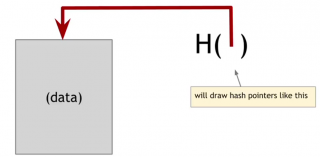
\includegraphics[scale=0.6]{hash_pointer}
\caption{Hash pointer}
\end{figure}

Iz definicije se vidi hash pointer nije ništa revolucionarno novo već samo pametna kombinacija alata koji su postojali i prije. Primjetimo da se sami podaci ne moraju kriptirati, što je ogromna prednost jer nama sama hash vrijednost podataka garantira da nije bilo promjena (naravno to daje uvjet da hash vrijednost bude sigurno spremljena). Također hash pointeri su toliko jednostavna struktura da ju možemo koristiti u implementaciji već poznatih većih struktura podataka (lista, binarno stablo i sl). Upravo tako je napravljen blockchain čiji je prikaz na slici \ref{fig:blockchain}).

\begin{figure}[!]
\centering
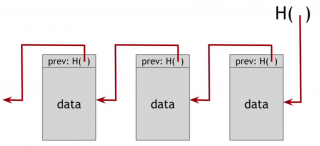
\includegraphics[scale=0.8]{blockchain}
\caption{Blockchain}
\label{fig:blockchain}
\end{figure}

Blockchain (u smislu strukture podataka) je vezana lista čije su veze hash pointeri. Očita razlika od obične vezane liste koja prozilazi iz toga da je veza hash pointer jest u tome da svaki blok sadrži informacije ne samo o sebi, već i o prijašnjem bloku. 

Kombinacija transparentnosti i nepromjenjivosti, koja je spomenuta u definiciji \ref{def:block}, postignuta je pametnim korištenjem hash pointera. Da to dokažemo trebamo se zapitati što bi se desilo kada bi napadač htio promjeniti neki podatak sadržan u blockchinu. Recimo da se taj podatak nalazi u bloku indexa $k$. Ako napadač promjeni sadržaj tog bloka, tada će se razlikovati i njegova hash vrijednost, a upravo ta hash vrijednost se nalazi u bloku $k+1$. Što znači da će napadač promjeniti i sadžaj bloka $k+1$, tj. promjeniti i njegovu hash vrijednost itd. Dakle vidimo ako napadač želi sakriti svoju jednu promjenu u podacima trebat će mjenjati sve blokove koji dolaze nakon bloka u kojem je nastala promjena. Znači pod uvjetom da \textbf{sigurno spremimo hash pointer samo zadnjega bloka} možemo garantirati za ispravnost sadržaja cijelog blockchaina. No u prethodnoj definiciji blockchain je naveden kao distribuirano spremište podataka i u takvoj situaciji nije praktično da svaki čvor mreže na kojoj se nalazi blockchain mora spremati hash poiner zadnjeg bloka jer mreža je asinkrona i lanac nije svugdje iste duljine. Tada ako uzimamo da je najdulji lanac uvijek ispravan, tj. ako je 50\% mreže iskreno tada također možemo garantirati da je blockchain siguran. Također zbog svojstva distribuiranosti i lakšeg transaporta po mreži valjalo bi i ograničiti veličinu bloka. No danas, memorija nije skup resurs, tako da u teoriji u blockchain zapravo možemo spremati podatke proizvoljne veličine.

\section{Bitcoin}

U jednostavnoj tehničkoj definiciji Bitcoin je zapravo jedan blockchain koji sadrži popis svih transakcija koje su se ikada desile. Taj blockchain je povezan u peer-to-peer mrežu. Svaki čvor mreže ima svoju kopiju blockchaina. On ju redovito održava i osvježuje u komunikaciji sa susjednim čvorovima. Pojedini čvor ne zna tko su mu susjedi i svaku informaciju koju dobije provjerava za sebe. U slučaju da od susjeda dobije blockchaine različitog sadržaja, zbog takve implementacije protokola, uvijek je blockchain najveće duljine garantirano točan. Ključna stvar koja se postiže u ovakvoj definiciji je decentralizacija. Na mreži žive accounti koji razmjenjuju tokene (Bitocoine) između sebe. Jedini način kako accounti komuniciraju je preko transakcija koje se zapisuju na blockchain. 

Ovo je sve što ću općenito reći o Bitcoinu i jedino ću detaljnije predstaviti 3 stvari koje će mi kasnije koristiti u ovom radu: identifikacija accounta na mreži, transakcije i transakcijske skripte. Prvo ću dati rješenje \textbf{decentraliziranog sustava identifikacije} accounta na mreži. U prethodnom dijelu smo dali definiciju digitalnog potpisa koji služi za autorizaciju u digitalnom svijetu, no on sam od sebe nije dovoljan za idenitifikaciju jer bi također trebali imati centralnu jedinicu koja će upravljati ključevima. Bitcoin problem identifikacije rješava zanimljivim trikom da gleda na javni ključ iz sheme digitalnog potpisa kao identitet accounta, točnije za to koristi već spomenuti digitalni potpis ECDSA. Posljedica uzimanja javnog ključa kao digitalnog identiteta accounta jest da fizička osoba koja kontrolira account (dakle posjeduje privatni ključ) nije nikako vezana za njega, već si može generirati novi par ključeva i stvoriti si novi account kada god poželi. Također već smo rekli da u ECDSA ključevi su proizvoljni 256-bitni niz nula i jedinica i nema nikakve sanše da se account poveže sa fizičko osobom tako da imamo i prilično veliku razinu anonimnosti na mreži.

Sada kada imamo sustav identifikacije možemo opisati kako Bitcoin implementira transakciju izmjeđu accountova. Transakcija je običan JSON objekt koji se vidi na slici \ref{fig:transakcija} koji se sastoji od 3 glavna dijela:
\begin{enumerate}
    \item \textit{metapodaci} - jedini bitan dio metapodataka nam je hash cijele transakcije, koji služi kao ID transakcije
    \item\textit{ulazne transakcije} - blockchain ne sadrži informaciju koliko pojedini account sadrži coina, već se svaka transakcija referencira na neku prijašnju u kojoj je taj account sudjelovao
    \item \textit{izlazni podaci} - izlazna vrijednost transakcije i \textbf{transakcijska skripta}
\end{enumerate}

\begin{figure}[h]
\centering
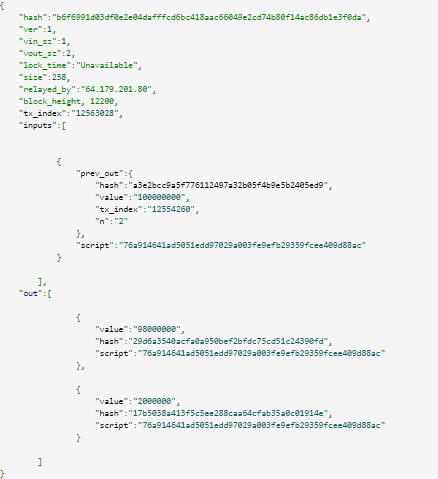
\includegraphics[scale=0.9]{transakcija}
\caption{Bitcoin transakcija}
\label{fig:transakcija}
\end{figure}

Nama najzanimljiviji dio transakcije je transakcijska skripta. Pod tim pojmom mislimo na računalni program pisan u jeziku Script. Taj program se izvršava prilikom prvog procesiranja transakcije i zapisivanju na blockchain te na ostalim čvoroima prilikom osvježavanja blockchaina. Kod toga programa se sam generira i nije programibilan. 

Script\cite{script} je programski jezik napravljen specifično za Bitcoin. Izvršava se na stogu, vrlo je jednostavan (ima mjesta za samo 256 naredbi, tj svaka naredba je kodirana u 2 broja u heksadecimalnom zapisu), nije Turing-kompletan i nema petlji.

\chapter{Ethereum}

Dok je Bitcoin zamišljen za specifičnu svrhu decentraliziranog izvršavanja financijskih transakcija, 2013. godine Vitalik Buterin je u svoj radu\cite{eth_paper} predstavio svoju ideju za novu generaciju blockchaina nazvanu Ethereum čiji je cilj izvršavanje proizvoljnih programa, tj. smart contracta. U ovom poglavlju ću predstaviti Ethereum i pokušati objasniti napredak u odnosu na svoje prethodnike.

\section{Općenito ili neki fora naziv}

S obzirom da mnogo ljudi dolazi do Ethereuma sa nekim prijašnjim iskustvima i znanjem o Bitcoinu, želim odmah na početku naglasiti razlike s obzirom da svoje prethodnike, pa po \cite{ethbook}:

\begin{definicija}
\textit{Ethereum} je open source, \textbf{globalno distribuirana računalna mreža} koja izvršava programe zvane smart contracti. Mreža koristi blockchain za sinkronizaciju i spremanje promjena stanja na mreži, a valutu zvanu \textbf{ether} za mjerenje i ograničavanje resursa mreže.
\end{definicija}

Vidimo odmah da je namjera ove definicije predstaljanje Ethereum kao mreže koja će biti pošlužitelj smart contractima, tj. decentralizirana platforma za aplikacije, a digitalna valuta je samo sredstvo koje se koristi da bi mreža ispravno funkcionirala. Zbog toga bi se moglo zaključiti da građa Ethereuma potpuno drukčija od ostalih kriptovaluta no iznenađujuće, to uopće nije slučaj.

I dalje je to u srcu blockchain sa potpuno istim kriptografskim alatima kao i kod Bitcoina, no stvar zbog koje je Ethereum bitno napredniji od svih svojih prethodnika je komunikacijski protokol. Bitcoinov komunikacijski protokol je bio prilično jednosmjeran, jedino su se mogle izvršavati transakcije koje su izmjenjivale tokene između acconta. Sa Ethereumovim komunikacijskim protokolom moguće je napisati proizvoljan program sa custom logikom, staviti ga u transakciju i poslati ga da se izvršava na mrežu. Taj program se naziva \textbf{smart contract}, a cijeli proces nam omogućuje \textbf{Ethereum Virutal Machine} u kojem se izvršava kod tog programa. Ethereum Virtual Machine (kao i svaki Virtual machine) je sloj apstrakcije između koda koji se izvršava i fizičkog računala koje izvšava kod, tj. sloj koji programski kod pisan u high-level jezicima preslikava u low-level \textbf{bytecode} (primjer \ref{eq:bytecode}).

\begin{napomena}
Low-level jezik je zapravo niz nul i jedinica razumljivih računalu koje ih izvodi, ali nama ljudima ne znači previše. Suprotno od toga postoje high-level jezici koji imaju snažnu ogradu od apstrakcije na koji računalo izvodi programe.
\end{napomena}

\begin{dmath}
0x608060405234801561001057600080fd5b5061018e806100206000396000f3\\fe608060405260043610610041576000357c0100000000000000000000000000\\000000000000000000000000000000900463ffffffff1680631e2aea0614610\\046575b600080fd5b34801561005257600080fd5b50610109600480360360208\\1101561006957600080fd5b8101908080359060200190640100...
\label{eq:bytecode}
\end{dmath}

\section{Accounti}

Princip identifikacije na mreži je također potpuno isti kao i prije, koristi se javni ključ iz sheme digitalnog potpisa ECDSA za identifikaciju uz jednu veliku razliku. Na Ethereumu postoje dvije vrste accounta: 
\begin{enumerate}
    \item User accounti
    \item Contract accounti
\end{enumerate}

\begin{figure}[h]
\centering
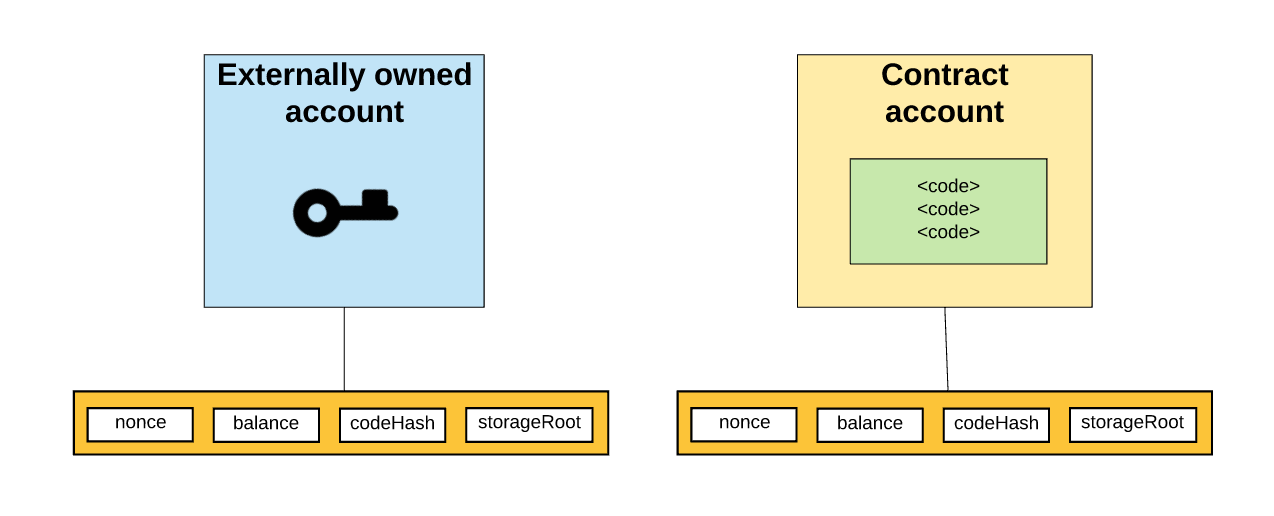
\includegraphics[scale=0.3]{ethaccounts}
\caption{Accounti na Ethereumu}
\label{fig:ethaccounts}
\end{figure}

Kod Bitcoina je ponašanje svakog accounta je bilo kontrolirano od strane neke fizičke osobe koja posjeduje privatni ključ od tog accounta, tj. postojali su samo User accounti. Ovdje postoji i drugi tip accounta, a to su adrese na kojima žive smart contracti. Kao što se vidi sa slike \ref{fig:ethaccounts} izvana su ti accounti jednaki (oba sadrže ether), jedina razlika jest što ponašanje accounta na čijoj je adresi smart contract, definirano pomoću koda koji se nalazi u njemu.

Kao i kod Bitcoina svaki čvor na mreži izvršava sve poslane transakcije i zapisuje stanje cijele mreže. S obzirom da bilo koji user account može napisati smart contract i poslati ga na mrežu, a nisu svi user accounti pouzdani, može doći do pretjeranog iskorištavanja resursa čvorova na mreži, npr. u slučaju da smart contract koji ima napisan \textbf{halting problem} bude poslan na mrežu, cijela mreža nebi nikad procesirala nijednu drugu transakciju. Zbog toga je uveden sustav naplate feeja za izvršvanje svakog koraka u kodu transakcije i taj sustav ćemo promotriti u idućem dijelu.

\section{Gas}

Na mreži Ethereum postoje dva tokena zvani: \textbf{ether} i \textbf{gas}. Ether ne trebamo pretjerano objašnjavati jer je to zapravo digitalna valuta koja se nalazi na Ethereumu i ima fizičku protuvrijednost (na Ether zapravo većina ljudi misli kada se kada spomene Ethereum), dok je gas sredstvo, tj. cijena izvršavanja transakcija i rada mreže. Vrijednost gasa se izvršava preko ethera te taj broj nije fiksan.

\begin{tcolorbox}
Već u samom imenu gas vidimo analogiju sa stvarnim svijetom. Možemo zamisliti gas kao benzin, novac kao ether, a auto kao cijelu Ethereum mrežu. Novcem kupujemo benzin koji je neophodan da bi auto radio. Isto tako ovdje etherom kupujemo gas koji je neophodan da bi Ethereum mreža radila, tj. procesirala transakcije i zapisivala ih na blockchain.
\end{tcolorbox}

Uz svaku transakciju koja se šalje na mrežu, account koji ju šalje treba postaviti dvije vrijednosti:

\begin{itemize}
    \item \textbf{Gas limit} - maksimalna količina gas-a koju transakcija smije potrošiti na svoje izvršavanje
    \item \textbf{Gas price} - vrijednost 1 gasa u etheru
\end{itemize}

Dakle dobivamo da je ukupna maksimalna vrijednost transakcije:
\begin{equation}
    MaxVrijednostTransakcije = GasLimit \times GasPrice
\end{equation}

Kažemo maksimalna vrijednost transakcije jer ne znamo za sve transakcije točan iznos s obzirom da možemo slati proizvoljan kod koji može ovisiti o argumentima koje pošaljemo. U slučaju da nije potrošen puni iznos koji smo naveli tada se ostatak vraća pošiljatelju, ali u slučaju da transakcija nije prošla (npr. nedovoljan iznos na računu) potrošeni gas pošiljatelj neće dobiti natrag. Potrošeni iznos gasa (dakle ethera) će dobiti čvor koji prvi izvrši transakciju i zapiše ju transakciju na blockchain. Primjetimo da mi sami određujemo koliko ćemo platiti jedinicu gasa, tj. ukupnu vrijednost koliko smo spremni platiti transakciju. S obzirom da čvorovi koji procesiraju transakcije sami odbiru koje će transakcije procesirati, vrlo je vjerojatno što veći iznos stavimo za cijenu gasa i samim time povećamo joj vrijednost, da će nam transakcija brže biti izvršena i zapisana na blockchain.

Također primjetimo da cijelo vrijeme govorimo transakcije i iako pod tim mislimo zapravo kod koji se izvršava, zapravo izraz transakcija je ispravan jer se kao i kod Bitcoina jedino pomoću njih mjenja stanje mreže i pokreću programi.

Sada kada imamo objašnjenu naplatu izvršavanja transakcija, promotrit ćemo primjere iz stvarnog svijeta koliko je skupo održavati aplikaciju na Ethereumu. Na slici \ref{fig:ethunits} se nalazi tablica pretvaranja jedinica ethera.

Primjeri za gas price u "standardnim" uvjetima: 
\begin{itemize}
    \item 40 GWEI - gotovo je sigurno da će transakcija biti zapisana u idući blok (vrijeme potrebno za 1 blok je u prosjeku 13 sekundi)
    \item 20 GWEI - prosjek, gotovo sigurno će transakcija biti zapisana u idućih par blokova
    \item 2 GWEI - gotovo sigurno će transakcija biti procesirana u idućih par minuta
\end{itemize}

\begin{figure}[!]
\centering
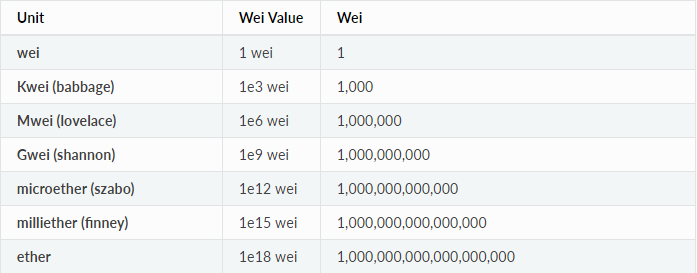
\includegraphics[scale=0.55]{ether_units}
\caption{Pretvorba jedinica ethera}
\label{fig:ethunits}
\end{figure}

Kao što smo prije napomenuli, svaki program se pomoću EMV-u kompajlira u bytecode. Bytecode sadrži samo jednostavne operacije koje različitu cijenu izvođenja (izraženu u gas-u) ovisno o tome koliko je pojedina operacija kompleksna. Tako na primjer postoje ADD što je najobičnije zbrajanje 2 broja koje košta 3 gasa, MUL je množenje i košta 5 gasa. Također postoje i malo kompleksnije operacije tipa BALANCE koje dohvaća iznos ethera koji pojedina adresa sadrži košta 700 gasa.

iiii jos neki primjeri jednostavnih programa koje cu tu navesti za dalje, sad sam samo ovaj dio koda jer mi je trebao za kasnije

\begin{minipage}{\linewidth}
\begin{lstlisting}[caption = Primjer 1, language=solidity, label={lst:suma}]
function sumArray(uint[] memory arrayToSum) pure returns (uint _sum) {
    _sum = 0;
    for (uint i = 0; i < arrayToSum.length; i++) {
        _sum += arrayToSum[i];
    }
}
\end{lstlisting}
\end{minipage}

\chapter{Smart Contracts}

U prvom poglavlju smo krenuli od najosnovnije kriptografije i blockchaina, kasnije ukratko predstavili Bitcoin te na kraju elemente Ethereuma. U ovom poglavlju ću napokon objasniti kako funkcionira sam smart contract, njegove mogućnosti i na kraju pogledati sigurnost.

\section{EMV \& Solidity}

Kao što smo rekli smart contract se izvodi u Ethereum Virtual Machinu (skraćeno EVM). EVM je stack-based virtual machine (izvršava sve operacije na stogu). Kompletno je izoliran od računala na kojem se nalazi (što znači da nema pristup filesystemu, mreži, okolini i sl.), ima neograničenu memoriju, ali što se više više memorije koristimo to više nas košta gasa, dakle granice u EVMa nisu statične već ekonomske. Da bi dobili bytecode koji EVM zna čitati, trebamo imati neki high level jezik koji je čitljiv nama ljudima, a može se prevesti u njega. Primjera takvih jezika je mnogo: Vyper, Bamboo, LLL, ali najpopularniji među njima je \textbf{Solidity}. Dizajniran specifično za pisanje smart contracta, Solidity je objektno orjentirani \textbf{Turing potpun} jezik vrlo sličan Javascriptu.

\begin{napomena}
Turing potpunost znači da se može izvršiti program proizvoljne kompleksnosti uz neograničenu memoriju.
\end{napomena}

Upravo u toj Turing potpunosti se vidi velik napredak u odnosu na Bitcoin, jer ako se prisjetimo Bitcoinova transakcijska skripta može samo izvršiti razmjenu tokena između accounta. Također valja napomenuti da nemaju svi gore navedeni jezici iste karakteristike, npr. Vyper nije uopće Turing potpun, ali zabog tih smanjenih mogućnosti mu je sigurnost puno veća.

\section{Pozivanje koda ili neki fora naziv}

Kao na Bitcoinu, svaka promjena stanja na Ethereumu zahtjeva slanje neke transakcije. Pri svakom slanju moramo specificirati adresu primatelja i sadržaj transakcije, što je prilično očekivano. Rekli smo da na Ethereumu postoje dvije vrste accounta: user i contract accounti. Ako smo specificirali da poruku prima user account tada sve što ta transakcija radi je prebacuje ether, no ako smo specificirali contract account tada aktiviramo smart contract i počinje se izvršavati kod. Smart contract \textbf{nema stanje} i slanjem transakcija je jedino moguće aktivirati ga (ovaj dio je naglašen jer to znači da je nemoguće imati funkcije koje se same pokreću, npr. periodičke funkcije ili jobovi). Kod smart contracta može:

\begin{itemize}
    \item Slati ether na željene adrese
    \item Čitati/pisati iz svoje memorije
    \item Pozivati izvršavanja drugih smart contracta
\end{itemize}

Znamo da se contract piše u nekom high-level jeziku koji se onda kompajlira u bytecode. Taj bytecode se zatim objavljuje na Ethereum mrežu tako da se pošalje transakcijom (kao transakcijska skripta) na adresu koja još nije iskorištena i kada je na mreži se pokreće ponovnim slanjem nove transakcije na tu adresu. No kako pozvati točno određenu funkciju na contractu? Pri kompajliranju smart contracta dobijemo mnogo informacija: bytecode,  \textbf{Application Binary Interface} (skraćeno ABI), potpis i ostale ovdje nebitne informacije.

\begin{definicija}
ABI je interface između dva programska modula, od kojih jedan je često na nivou strojnog koda (niz nula i jedinica), a drugi program kojeg pokreće čovjek.
\end{definicija}

U kontekstu Ethereuma, ABI je popis svih funkcija koje se koriste u contractu (a mogu biti pozvane izvan njega) zajedno sa argumentima i povratnim tipovima. Pozivanje funkcije se odvija tako da se djelovi ABIja zajedno sa argumentima funkcije kodiraju u bytecode koji se kasnije ubaci u transakciju za slanje.

\begin{figure}[!]
\centering
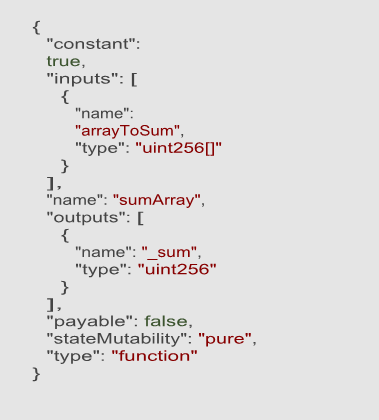
\includegraphics[scale=0.7]{abi}
\caption{Primjer ABI-ja}
\label{fig:abi}
\end{figure}

Na slici \ref{fig:abi} se nalazi ABI funckije iz primjera \ref{lst:suma} koja računa zbroj svih elemenata polja. Ako želimo pozvati tu funkciju $sumArray([164, 46])$ tada bi poslali ukupno 36 bytova koji izgledaju: 


\begin{dmath}
\label{eq:sumabi}
    0x1e2aea06a40000000000000000000000000000000000000000000\\00000000000000000002e000000000000000000000000000000000\\00000000000000000000000000000
\end{dmath}

Taj kod nam ne znači previše, ali ako razdvojimo na svoje djelove dobijemo: 

\begin{itemize}
    \item Prvih 4 bytea je ID funkcije. ID se dobije tako da se uzme početak hash vrijednosti potpisa funkcije, tj. u ovom slučaju primjeni Keccak256 hash funkcija na $arraySum(uint256[])$
    \begin{equation*}
        h(arraySum(uint256[])) = \textbf{1e2aea06}47440989b12156a7890618f416...
    \end{equation*}
    \item Ostatak su argumenti funkcije. Uvijek je to zapravo njihova hex vrijednost proširena da ima veličinu 32 byta. S obzirom da je ovdje polje brojeva u pitanju proširenje s nulama će doći s desne strane hex vrijednosti.
    \begin{equation*}
        paddedHex(164) = 0xa400000000000000000000000000000000000000...
    \end{equation*}
        \begin{equation*}
        paddedHex(46) = 0x2e000000000000000000000000000000000000000...
    \end{equation*}
\end{itemize}

Algoritam takvog kodiranja se zove \textbf{Recursive Length Prefix} i kompleksniji primjeri se nalaze na \cite{rlp}.

Još samo za kraj ću napraviti provjeru da nisam pogriješio u algoritmu. Naime smart contract koji se nalazi u primjeru \ref{eq:bytecode} sadrži upravo funkciju $sumArray$ i što znači da taj bytecode mora imati potpis te funkcije ($1e2aea06$), a to je istina.

\begin{dmath}
0x608060405234801561001057600080fd5b5061018e806100206000396000f3\\fe608060405260043610610041576000357c0100000000000000000000000000\\000000000000000000000000000000900463ffffffff168063\textcolor[rgb]{1,0,0}{1e2aea06}14610\\046575b600080fd5b34801561005257600080fd5b50610109600480360360208\\1101561006957600080fd5b8101908080359060200190640100...
\label{eq:bytecode}
\end{dmath}

\section{Sigurnost}

U ovom trenutku postoji više od 1 000 000 smart contracta na Ethereumu koji skupa posjeduju preko 100 000 000 Ethera (trenutna cijena jednog Ethera je 349\$) u sebi. Zbog takovg kapitala koji trenutno posjeduju posebno su zanimljivi hakerima. Smart contracti su nova tehnologija i već kao takva daju izazove jer nema standardiziranog principa razvoja. Također, objavljeni su na blockachainu i jednom kada se pošalju na mrežu ne mogu se mjenjati i nadograđivati tako da svaka greška ostavlja trajne posljedice. Primjer jedne takve greške je \textbf{DAO hack} (dio koda koji je hakiran je na primjeru \ref{lst:hack}) koji se dogodio 2016. godine u kojem je ukradeno 50 000 000\$ i zbog kojega se Ethereum blockchain morao napraviti razdvajanje na dva lanca. Napravljen je novi lanac čije je stanje jednako onome prije hacka (dakle vraćene su sve transakcije) i danas je to Ethereum, dok je lanac na kojem se dogodio hack nastavio živjeti i danas se on zove Ethereum Classic.

\begin{minipage}{\linewidth}
\begin{lstlisting}[caption = Ukratko: DAO je jedna od drugih valuta na Ethereumu koja je imala svoju protuvrijednost u Etheru. Funkcija witdraw jednostavno povlači sredstva koje account ima na smart contractu. No što ako damo hrpu zahtjeva odjednom? Tada se sredstva konstantno prebacuju na account no na smart contractu se ne stigne smanjiti, language=solidity, label={lst:hack}]
function withdraw(uint _amount) public {
  if(balances[msg.sender] >= _amount) {
    if(!msg.sender.call.value(_amount)()) { 
        throw;
    }
    balances[msg.sender] -= _amount;
  }
}
\end{lstlisting}
\end{minipage}

Još jedno ograničenje koje je bitno jest naplata izvođenja koda, dakle funkcionalnost je "bitnija" od sigurnosti. To izvođenje znamo da se vrši iz bytecoda na koji mi imamo jedini utjecaj preko high-level jezika u kojima pišemo smart contracte. Dakle njihova sigurnost zapravo proizlazi iz sigurnosti samog jezika u kojem pišemo.

Solidity je Turing potpun jezik rađen po uzoru na Javascript, a Javascript nije poznat kao siguran jezik. Dakle i Solidity ima standardne probleme kao što su overflow i underflow. No Solidity strašno brzo napreduje i (službeno po Githubu 315 ljudi ga razvija i od prosinca 2015. je doživio 59 izdanja) popravlja probleme svakim novim izdanjem no i dalje postoje sumnje u Solidity kao pravi jezik za smart contracte. Upravo se mnogo ljudi zalažu za neke Turing nepotpune jezike poput Vypera koji mogu većinu operacija izvesti kao i Solidity no mnogo su sigurniji.

Još bi samo htio na kraju reći malo o sigurnosti s legalne strane. Naime trenutno nigdje ne postoji niti jedan članak zakona kojim bi se smart contracti predstavljali kao zakonski ugovor (ili barem nešto slično tome) što je prilično interesantna činjenica s obzirom da ima toliki ogroman kapital pohranjen u sebi.
    
\chapter{Primjer: Crypto Roullete}

\begin{figure}[h]
\centering
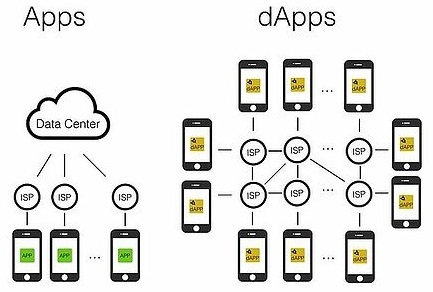
\includegraphics[scale=0.55]{AppsVSdApps}
\caption{Apps VS. dApps}
\label{fig:appvsdapp}
\end{figure}

\begin{figure}[h]
\centering
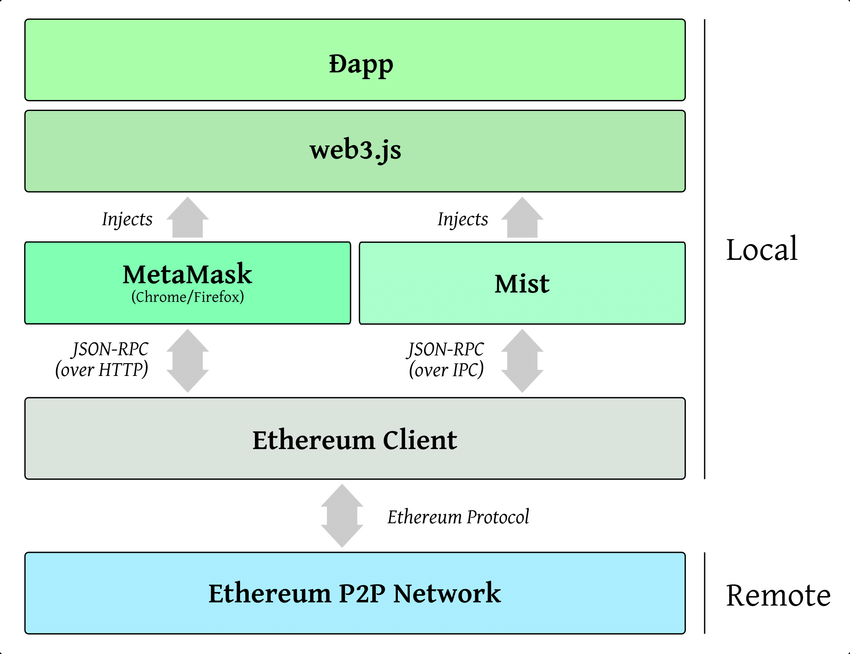
\includegraphics[scale=0.4]{dapp-architecture}
\caption{dApp architecture}
\label{fig:dapp}
\end{figure}

\chapter{Zaključak}

https://www.coindesk.com/axa-using-ethereums-blockchain-new-flight-insurance-product

\printbibliography

\end{document}
